\documentclass{article}
\usepackage[margin=1in]{geometry}
\usepackage{tikz}
\usetikzlibrary{positioning,arrows.meta,shapes,shadows.blur}
\usepackage{tcolorbox}
\usepackage{fontawesome5}
\usepackage{xcolor}

\newcommand{\benchmark}{ChemChain}

\begin{document}

\begin{figure}[t]
    \centering

    % VERSION 4: Modern Streamlined Flow
    \begin{tcolorbox}[
        title=\textbf{Chemistry: Reaction Cascade} \hfill {\small\colorbox{teal!20}{Medium} \quad 9 steps},
        colframe=teal!70!black,
        colback=white,
        boxrule=0.8pt,
        width=\textwidth
    ]
    \small
    \begin{tikzpicture}[remember picture, overlay]
        \node[opacity=0.04, anchor=east] at ([xshift=-0.35cm, yshift=0.1cm]current page.east) {\Huge\faFlask};
    \end{tikzpicture}

    \textbf{Dependency graph:}
    \begin{center}
    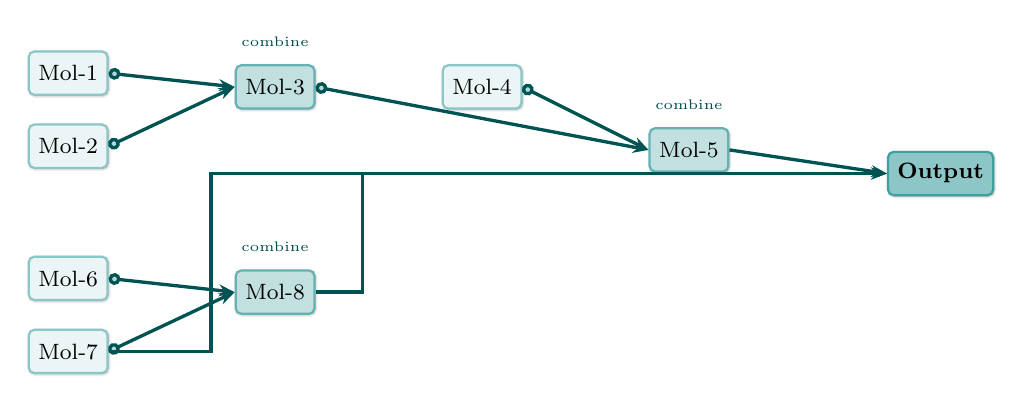
\begin{tikzpicture}[
        node distance=0.65cm and 0.95cm,
        mol/.style={
            draw,
            rounded corners=2pt,
            minimum width=1.0cm,
            minimum height=0.55cm,
            thick,
            font=\footnotesize,
            blur shadow={shadow blur steps=5, shadow xshift=0.3pt, shadow yshift=-0.3pt, shadow blur radius=1pt}
        },
        molinput/.style={mol, fill=teal!8, draw=teal!45},
        molstep/.style={mol, fill=teal!24, draw=teal!60},
        moloutput/.style={mol, fill=teal!45, draw=teal!75, font=\footnotesize\bfseries},
        arr/.style={-{Stealth[length=2mm]}, line width=1.2pt, teal!65!black},
        merge/.style={{Circle[length=1.5mm, fill=teal!30]}-{Stealth[length=2mm]}, line width=1.2pt, teal!65!black}
    ]
        % Inputs arranged in two groups
        \node[molinput] (m1) {Mol-1};
        \node[molinput, below=0.35cm of m1] (m2) {Mol-2};

        \node[molinput, below=1.1cm of m2] (m6) {Mol-6};
        \node[molinput, below=0.35cm of m6] (m7) {Mol-7};

        % First level products
        \node[molstep, right=1.6cm of m1.east, yshift=-0.175cm] (m3) {Mol-3};
        \node[molstep, right=1.6cm of m6.east, yshift=-0.175cm] (m8) {Mol-8};

        % Second input
        \node[molinput, right=1.6cm of m3.east] (m4) {Mol-4};

        % Second level product
        \node[molstep, right=1.6cm of m4.east, yshift=-0.8cm] (m5) {Mol-5};

        % Final output
        \node[moloutput, right=2.0cm of m5.east, yshift=-0.3cm] (final) {Output};

        % Arrows - merge arrows for combinations
        \draw[merge] (m1.east) -- (m3.west);
        \draw[merge] (m2.east) -- (m3.west);

        \draw[merge] (m6.east) -- (m8.west);
        \draw[merge] (m7.east) -- (m8.west);

        \draw[merge] (m3.east) -- (m5.west);
        \draw[merge] (m4.east) -- (m5.west);

        % Final connections
        \draw[arr] (m5.east) -- (final.west);
        \draw[arr] (m8.east) -| ([xshift=0.6cm]m8.east) |- (final.west);
        \draw[arr] (m7.east) -| ([xshift=1.3cm]m7.east) |- (final.west);

        % Reaction labels (small)
        \node[font=\tiny, teal!60!black, anchor=south] at ([yshift=0.1cm]m3.north) {combine};
        \node[font=\tiny, teal!60!black, anchor=south] at ([yshift=0.1cm]m8.north) {combine};
        \node[font=\tiny, teal!60!black, anchor=south] at ([yshift=0.1cm]m5.north) {combine};
    \end{tikzpicture}
    \end{center}

    \vspace{0.0cm}
    \begin{tabular}{@{}p{0.48\textwidth}p{0.48\textwidth}@{}}
    \textit{Sample step (Subproblem 3):} React Mol-1 + Mol-2 in THF at room temp. Predict major product. &
    \textit{Final step:} Count hydrogens in Mol-5, Mol-7, Mol-8. \\
    \end{tabular}

    \vspace{0.2cm}
    \hfill \textbf{Answer:} \texttt{[19, 15, 23]}
    \end{tcolorbox}

    \caption{\textbf{Version 4:} Streamlined modern design with subtle shadows and merge-point indicators (circles) showing where molecules combine. Clean white background emphasizes the flow structure.}
\end{figure}

\end{document}
